\documentclass[submission, Phys]{SciPost}
\usepackage[T1]{fontenc}
\usepackage[utf8]{inputenc}
\usepackage{amsmath,amssymb,bm,booktabs,graphicx,siunitx}
\graphicspath{{../figures/}}
\usepackage[nameinlink,capitalize,noabbrev]{cleveref}
\usepackage{xr}
\externaldocument[MAIN-]{SciPost_Chaos_Floquet_SyntheticFlux}
\sisetup{detect-all}

\newcommand{\dd}{\,\mathrm{d}}
\newcommand{\Tr}{\operatorname{Tr}}

\begin{document}

\begin{center}{\Large \textbf{
Supplementary Material: physical anchoring and matched measurement-Fisher reference for dissipative optomechanics with synthetic flux\\
}}\end{center}

\begin{center}
Stella Rolande Mbokop Tchounda\textsuperscript{1},
Carolle Tchodimou\textsuperscript{1},
Philippe Djorwe\textsuperscript{2},
Sifeu Takougang Kingni\textsuperscript{3} and
Serge Guy Nana Engo\textsuperscript{1$\star$}
\end{center}

\begin{center}
{\bf 1} Department of Physics, Faculty of Science, University of Yaound\'e I, P.O. Box 812, Yaound\'e, Cameroon
\\
{\bf 2} Department of Physics, Faculty of Science, University of Ngaound\'er\'e, P.O. Box 454, Ngaound\'er\'e, Cameroon
\\
{\bf 3} Department of Mechanical, Petroleum and Gas Engineering, National Advanced School of Mines and Petroleum Industries, University of Maroua, P.O. Box 46, Maroua, Cameroon
\\
${}^\star$ {\small \sf serge.nana-engo@facsciences-uy1.cm}
\end{center}

\begin{center}
\today
\end{center}

\section{Overview and reading guide}This Supplementary Material supports the main text by providing the
normalization, anchor selection, physically anchored reference table, the
matched measurement-Fisher reference tables and their observation-window
robustness check, the formal statements of the Lyapunov--Floquet consistency
criterion and the matched-measurement Fisher lemma (with their proofs), the
representative finite-time convergence of the strong-coupling spectrum, the
threshold sensitivity of the hyperchaos-order classification, the
reduced-model parameter screen, the amplitude-quadrature noise-model
cross-check against a quantum master equation, the matched measurement
Fisher calculation on the chaotic attractor and the semiclassical boundary of
the strong-coupling classification, and the explicit technical backup that
the Discussion in the main text compresses: a per-gap limitations statement,
a per-parameter feasibility audit against the silicon optomechanical anchor,
a per-seed robustness decomposition of the long-window trajectory audit, and
a phase-sweep and single-mode collapse of the matched Fisher on the chaotic
attractor. The reading order that follows the main text is: anchors
(\cref{SI-sec:anchor}); matched Fisher (\cref{SI-sec:matched-fisher});
theorems and proofs (\cref{SI-sec:theorems}); convergence
(\cref{SI-sec:convergence}); threshold sensitivity
(\cref{SI-sec:threshold-sensitivity}); observation-window check
(\cref{SI-sec:fisher-window}); reduced-model screen
(\cref{SI-sec:reduced-pareto}); noise cross-check
(\cref{SI-sec:noise-model-crosscheck}); interpretation
(\cref{SI-sec:interpretation}); attractor Fisher
(\cref{SI-sec:attractor-fisher}); semiclassical boundary
(\cref{SI-sec:semiclassical-boundary}); limitations and residual gaps
(\cref{SI-sec:limitations}); feasibility audit
(\cref{sec:feasibility-audit}); initial-condition robustness
(\cref{sec:initial-condition-robustness}); attractor-Fisher audit
(\cref{SI-sec:attractor-fisher-audit}). Every
quantitative claim in the main text is traceable to a table or
deterministic script invoked below.

\section{Normalization and anchor selection}
\label{SI-sec:anchor}

The main text uses a rotating-frame Hamiltonian normalized to a reference
mechanical frequency $\omega_m$, so that all rates and couplings are reported as
dimensionless ratios $x/\omega_m$. A physically anchored reference set is obtained by
fixing $\omega_m$ from a device with gigahertz mechanical modes and optically mediated
phonon coupling, and by reading the damping, decay, and coupling rates from the same
platform. The primary anchors and the model source are:

\begin{itemize}
\item \textbf{Mayor \emph{et al.}~\cite{Mayor2025}}: a silicon two-dimensional optomechanical
crystal with mechanical frequency $f_m = \SI{7.436}{\giga\hertz}$, mechanical quality
factor $Q_m = \num{3.6e4}$ (giving $\gamma_m/2\pi = f_m/Q_m = \SI{206.6}{\kilo\hertz}$),
cavity linewidth $\kappa/2\pi = \SI{800}{\mega\hertz}$, and single-photon
optomechanical coupling $g_0/2\pi = \SI{880}{\kilo\hertz}$.
\item \textbf{Mathew, del Pino and Verhagen~\cite{Mathew2020}}: a nano-optomechanical
implementation of synthetic gauge fields for phonon transport, whose demonstrated
coupling scale (a direct next-nearest-neighbour rate near $\SI{10}{\kilo\hertz}$ and an
optically mediated rate near $\SI{200}{\kilo\hertz}$ at a $\SI{2.4}{\mega\hertz}$
mechanical frequency, i.e. up to a few percent of $\omega_m$) bounds the
phase-controlled inter-resonator hopping $J_m$.
\item \textbf{Muthukumar \emph{et al.}~\cite{muthukumar2025doi}}: the model antecedent. The
present work retains the one-cavity/two-mechanical-resonator topology and
phase-dependent hopping, but not the numerical regime or detuning notation
unchanged. Muthukumar \emph{et al.} use
$\Delta_{\mathrm M}=\omega_L-\omega_c$ and report
$\kappa/\omega_m=\num{7.3e-2}$, $g/\omega_m=\num{1.077e-4}$,
$\gamma/\omega_m=\num{1.077e-5}$, $J_m/\omega_m=\num{2e-4}$,
$\omega_2/\omega_m=1+\num{5e-4}$, and
$\Delta_{\mathrm M}/\omega_m=1$ at
$\omega_m/2\pi\approx\SI{1}{\giga\hertz}$. In the convention of the present
manuscript, $\Delta=-\Delta_{\mathrm M}$. The reference reported bistability,
self-excited oscillations, and phase-selected chaotic regimes. The present analysis
uses $E=\sqrt{\kappa}\,\alpha^{\rm in}$, permits $g_1\neq g_2$, and examines a
strongly damped, strongly coupled sector that is not the resolved-sideband regime
of that reference.
\end{itemize}

\begin{table}[h]
  \centering
  \small
  \caption{Scope and parameter comparison with Muthukumar \emph{et al.}~\cite{muthukumar2025doi}.
  The topology and phase-dependent mechanical hopping are inherited; the detuning
  convention, coupling symmetry, and operating regime are stated explicitly so that
  the present calculations are not read as a parameter-for-parameter reproduction.}
  \label{tab:muthukumar-comparison}
  \begin{tabular}{@{}p{0.23\linewidth}p{0.31\linewidth}p{0.37\linewidth}@{}}
    \toprule
    Quantity & Muthukumar \emph{et al.} & Present manuscript \\
    \midrule
    Architecture & One optical cavity; two mechanically coupled resonators; phase-dependent $J_m$ & Same topology and hopping structure; six-dimensional semiclassical state \\
    Detuning convention & $\Delta_{\mathrm M}=\omega_L-\omega_c$, with $\Delta_{\mathrm M}/\omega_m=1$ & $\Delta=\omega_c-\omega_L=-\Delta_{\mathrm M}$; present reference uses $\Delta/\omega_m=-1$ \\
    Cavity decay & $\kappa/\omega_m=\num{7.3e-2}$ & $\kappa/\omega_m=1$ in the validated reference and strong-coupling sectors \\
    Mechanical damping & $\gamma/\omega_m=\num{1.077e-5}$ & $\gamma_{1,2}/\omega_m=\num{0.02}$ \\
    Optomechanical coupling & Symmetric $g/\omega_m=\num{1.077e-4}$ & Weak reference: $(g_1,g_2)/\omega_m=(\num{0.02},\num{0.018})$; strong sector: $(\num{0.30},\num{0.27})$ \\
    Mechanical detuning & $\omega_2/\omega_m=1+\num{5e-4}$ & $\omega_2/\omega_m=\num{1.03}$ \\
    Inter-resonator hopping & $J_m/\omega_m=\num{2e-4}$ & $J/\omega_m=\num{0.08}$ in the main numerical sectors \\
    Drive coordinate & $\alpha^{\rm in}$, with $E=\sqrt{\kappa}\,\alpha^{\rm in}$ under the shared normalization & $E=\num{0.2}$ for the stable reference; $E=\num{4}$--$\num{8}$ for the chaotic/hyperchaotic sectors \\
    Primary result & Bistability, self-excited oscillations, and phase-selected chaos; sensing proposal & Full six-exponent classification, drive/coupling-gated transition, Neimark--Sacker onset, and matched Fisher bound \\
    Experimental status & Resolved-sideband, literature-model scenario & Strong sector is explicitly model-level; no calibrated device prediction is claimed \\
    \bottomrule
  \end{tabular}
\end{table}

\section{Physically anchored reference set}

\Cref{tab:si-calibrated} summarizes the reconciled reference set. The single-mode
parameters ($\omega_m$, $\kappa$, $\gamma_m$, $g_0$) are anchored to Mayor
\emph{et al.}; the inter-resonator hopping $J_m$ is scanned over a range bounded by the
Mathew \emph{et al.} coupling scale, because no direct two-resonator gigahertz
measurement of the phase-controlled coupling is available. The cavity--laser detuning
$\Delta=\omega_c-\omega_L$ and the drive amplitude $E$ are not calibrated by either
anchor: $\Delta$ depends on the cavity and laser frequencies, and $E$ cannot be
converted to an input power without the pump frequency, the external coupling, and the
explicit input-field normalization.

\begin{table}[h]
  \centering
  \caption{Physically anchored reference parameter set for the one-optical/two-mechanical
  optomechanical model of the main text. Normalized values are in units of the
  reference mechanical frequency $\omega_m=2\pi\times\SI{7.436}{\giga\hertz}$. The
  reference operating point used for the numerical validation of the main text is shown for
  comparison and is not a calibrated device.}
  \label{tab:si-calibrated}
  \begin{tabular}{@{}lllll@{}}
    \toprule
    Quantity & Symbol & Normalized ($x/\omega_m$) & Value at $\omega_m$ & Basis \\
    \midrule
    Mechanical frequency (reference) & $\omega_m$ & $1$ & $2\pi\times\SI{7.436}{\giga\hertz}$ & Anchor \\
    Cavity decay rate & $\kappa$ & $\num{0.108}$ & $\SI{800}{\mega\hertz}$ & Measured \\
    Mechanical damping & $\gamma_m$ & $\num{2.78e-5}$ & $\SI{206.6}{\kilo\hertz}$ & Measured ($Q_m=\num{3.6e4}$) \\
    Optomechanical coupling & $g_0$ & $\num{1.18e-4}$ & $\SI{880}{\kilo\hertz}$ & Measured \\
    Inter-resonator hopping & $J_m$ & $[\num{1e-3},\num{1e-1}]$ & $[\SI{7.4}{\mega\hertz},\SI{744}{\mega\hertz}]$ & Scan \\
    \midrule
    Second mechanical mode & $\omega_2$ & $\num{1.03}$ & assumed near-degenerate & Assumed \\
    Cavity--laser detuning & $\Delta$ & free & --- & Free scan \\
    Drive amplitude & $E$ & normalized only & --- & Not convertible \\
    \bottomrule
  \end{tabular}
\end{table}

\begin{table}[h]
  \centering
  \caption{Comparison of the numerical-validation reference operating point with the
  physically anchored reference set. The reference point uses damping and coupling rates that are
  about one to three orders of magnitude larger than the anchored values, which is why
  it is reported as a model-level validation rather than a device prediction. The final
  column gives the feasibility judgment relative to the anchored platform; the
  strong-coupling hyperchaos sector is unreachable with the anchored optomechanical
  coupling.}
  \label{tab:si-pilot-vs-anchor}
  \begin{tabular}{@{}lcccc@{}}
    \toprule
    Quantity & Reference & Anchored & Ratio (reference / anchor) & Feasibility \\
    \midrule
    $\kappa/\omega_m$ & $\num{1.0}$ & $\num{0.108}$ & $\num{9.3}$ & challenging \\
    $\gamma_m/\omega_m$ & $\num{0.02}$ & $\num{2.78e-5}$ & $\num{720}$ & unreachable \\
    $g_0/\omega_m$ & $[\num{0.018},\num{0.02}]$ & $\num{1.18e-4}$ & $\approx\num{160}$ & unreachable \\
    $J_m/\omega_m$ & $\num{0.08}$ & $[\num{1e-3},\num{1e-1}]$ & within scan range & reachable \\
    \bottomrule
  \end{tabular}
\end{table}

\section{Matched measurement-Fisher reference for force sensing}
\label{SI-sec:matched-fisher}

The classical measurement Fisher information $F_C(F)$ of the main text is
computed for a weak external force $F$ on mechanical mode $1$ (a
momentum-quadrature drive), read out through the cavity amplitude quadrature
$X_a=\Re(\alpha)$ under matched drive $E=\num{0.2}$, observation time (one
drive period), detector noise (\num{0.01}), and thermal baths
($n_{\mathrm{th},1}=n_{\mathrm{th},2}=\num{0.1}$). \Cref{tab:si-matched-fisher}
lists $F_C(F)$ versus the synthetic-flux phase together with the two matched
references---the flux-off coupled sensor ($\theta=0$, $J=\num{0.08}$) and the
single-mode linear sensor ($J=0$)---and the gain relative to each.

\begin{table}[h]
  \centering
  \caption{Matched measurement Fisher information $F_C(F)$ for force sensing
  versus the synthetic-flux phase $\theta$, with the flux-off coupled reference
  ($\theta=0$, $J=\num{0.08}$) and the single-mode linear reference ($J=0$).
  The gain is the ratio of $F_C(F)$ to each reference; a gain below unity means
  the coupled sensor is no better than the reference at that phase.}
  \label{tab:si-matched-fisher}
  \begin{tabular}{@{}lcccc@{}}
    \toprule
    $\theta/\pi$ & $F_C(F)$ & Gain vs flux-off & Gain vs single mode \\
    \midrule
    $0$ & \num{4.503e-5} & \num{1.000} & \num{0.876} \\
    $1/4$ & \num{4.694e-5} & \num{1.042} & \num{0.913} \\
    $1/2$ & \num{5.191e-5} & \num{1.153} & \num{1.010} \\
    $3/4$ & \num{5.721e-5} & \num{1.271} & \num{1.113} \\
    $1$ & \num{5.958e-5} & \num{1.323} & \num{1.159} \\
    \midrule
    Flux-off reference & \num{4.503e-5} & \num{1.000} & \multicolumn{1}{c}{---} \\
    Single-mode reference & \num{5.141e-5} & \multicolumn{1}{c}{---} & \num{1.000} \\
    \bottomrule
  \end{tabular}
\end{table}

The central-difference estimate is converged with respect to the force step:
\Cref{tab:si-fisher-eps} lists $F_C(F)$ at the two flux extrema
($\theta=\pi/2$ and $\theta=\pi$) for force steps $\num{1e-5}$, $\num{1e-4}$,
and $\num{1e-3}$; the values agree to better than $\SI{0.01}{\percent}$. A
drive--temperature sweep (main text) further confirms that the gains are stable
across $E\in[\num{0.1},\num{1.0}]$ and $n_{\mathrm{th}}\in[0,1]$ to within
$\num{1e-3}$.

\begin{table}[h]
  \centering
  \caption{Convergence of the central-difference force-sensing Fisher
  information with the force step $\varepsilon$ at the two flux extrema.}
  \label{tab:si-fisher-eps}
  \begin{tabular}{@{}lccc@{}}
    \toprule
    $\varepsilon$ & $F_C(F)$ at $\theta=\pi/2$ & $F_C(F)$ at $\theta=\pi$ \\
    \midrule
    \num{1e-3} & \num{5.190751e-5} & \num{5.958194e-5} \\
    \num{1e-4} & \num{5.190938e-5} & \num{5.958166e-5} \\
    \num{1e-5} & \num{5.190763e-5} & \num{5.958181e-5} \\
    \bottomrule
  \end{tabular}
\end{table}

\paragraph{Optimized linear-sensor reference.}
The gains of \Cref{tab:si-matched-fisher} compare the flux sensor and the
single-mode reference at the same fixed readout $X_a=\Re(\alpha)$. To exclude
the possibility that the order-unity gain merely reflects a suboptimal
reference readout, the classical Fisher information is recomputed for the
rotated cavity quadrature
$X_\varphi=\Re(\alpha)\cos\varphi+\Im(\alpha)\sin\varphi$ with $\varphi$
optimized for each configuration. The optimal homodyne angle is
$\varphi_\star\approx\num{0.79}\pi$ for every configuration: it is fixed by
the linear cavity response ($\Delta=-1$, $\kappa=1$) and is independent of the
synthetic-flux phase, so readout optimization rescales $F_C$ by the same factor
(\num{1.56}) for the flux sensor and for both references. The flux-phase gain
relative to the single-mode linear reference is therefore unchanged under
readout optimization (\Cref{tab:si-optimized-readout}): it ranges from
\num{0.88} ($\theta=0$) to \num{1.16} ($\theta=\pi$), identical to the
matched-readout gains of \Cref{tab:si-matched-fisher} to within \num{1e-3}.
The order-unity gain is consequently not an artifact of a suboptimal reference
readout; it is a small, readout-robust linear-response effect of the
phase-controlled mode coupling, with no quantum advantage.

\begin{table}[h]
  \centering
  \caption{Readout-optimized classical Fisher information $F_C(F)$ for force
  sensing. $X_a$ is the matched amplitude quadrature
  $\Re(\alpha)$; $\varphi_\star$ is the optimal homodyne angle and
  $F_C(\varphi_\star)$ the corresponding value. The final column is the gain
  relative to the optimized single-mode reference ($J=0$, $\varphi_\star=\num{0.79}\pi$),
  and equals the matched-readout gain of \Cref{tab:si-matched-fisher} to within
  \num{1e-3}.}
  \label{tab:si-optimized-readout}
  \begin{tabular}{@{}lccccc@{}}
    \toprule
    $\theta/\pi$ & $F_C(X_a)$ & $\varphi_\star/\pi$ & $F_C(\varphi_\star)$ & Gain vs optimized single mode \\
    \midrule
    $0$ & \num{4.503e-5} & \num{0.79} & \num{7.033e-5} & \num{0.876} \\
    $1/4$ & \num{4.694e-5} & \num{0.79} & \num{7.331e-5} & \num{0.913} \\
    $1/2$ & \num{5.191e-5} & \num{0.79} & \num{8.108e-5} & \num{1.010} \\
    $3/4$ & \num{5.721e-5} & \num{0.79} & \num{8.937e-5} & \num{1.113} \\
    $1$ & \num{5.958e-5} & \num{0.79} & \num{9.306e-5} & \num{1.159} \\
    \midrule
    Single-mode reference & \num{5.141e-5} & \num{0.79} & \num{8.030e-5} & \num{1.000} \\
    \bottomrule
  \end{tabular}
\end{table}

\section{Lyapunov--Floquet consistency theorem and matched-measurement Fisher lemma}
\label{SI-sec:theorems}
\label{sec:theorems}

\paragraph{Theorem (Lyapunov--Floquet consistency criterion).}
Consider a drive-locked periodic orbit $x_p(t+T)=x_p(t)$ of the
phase-augmented system, with monodromy $M(T)$ and QR/Benettin spectrum~\cite{benettin1980,wolf1985,eckmann1985}
$\{\lambda_i\}$. Suppose the Floquet rates $\rho_i=T^{-1}\ln|\mu_i|$ (with
$\mu_i=\mathrm{eig}_i[M(T)]$) agree with the QR exponents within a fixed
tolerance $\delta_{\rm tol}$, and the divergence sum satisfies
\begin{equation}
 \sum_i\lambda_i=\frac1T\int_0^T\operatorname{tr}J(x_p(t),t)\,\dd t
 +\mathcal{O}(\delta_{\rm tol}),
\label{eq:divergence-theorem}
\end{equation}
with the phase direction treated explicitly. Then the orbit is exponentially
stable if and only if $|\mu_i|<1$ for all transverse multipliers, and in that
case $\lambda_{\max}<0$. The criterion is a consistency test, not an input
assumption: it certifies that the three independent diagnostics (monodromy,
Floquet rates, QR spectrum) describe the same linearization of the same
orbit. The measured values at the reference operating point (one-period orbit
residual $\num{9e-9}$, max Floquet--QR discrepancy $\num{2.68e-4}$, and
$\num{2.85e-4}$ across the
extended grid) satisfy the criteria and therefore
certify a stable periodic orbit---they do not by themselves certify a
flux-dependent transition, which is why the full-spectrum classification of the
main text is required.

\paragraph{Lemma (periodic covariance as an affine fixed point).}
Let $A(t)=J(x_p(t),t)$ be the Jacobian along the drive-locked orbit, $M(T)$ its
monodromy, and $Q(t)=B(t)N(t)B(t)^T$ the diffusion of the linearized Langevin
equation $\delta\dot x=A(t)\delta x+B(t)\eta$. Integrating the covariance
equation $\dot V=AV+VA^T+Q$ over one period gives the affine map
\begin{equation}
 \operatorname{vec}V(T)=[M(T)\otimes M(T)]\operatorname{vec}V(0)+q_T,
\label{eq:cov-affine}
\end{equation}
where $q_T$ collects the noise forcing propagated by the state-transition
matrix. A $T$-periodic covariance therefore solves the linear system
\begin{equation}
 [I-M(T)\otimes M(T)]\operatorname{vec}V(0)=q_T,
\label{eq:cov-fixed-point}
\end{equation}
whose solvability requires that no pair of Floquet multipliers satisfies
$\mu_i\mu_j=1$. This is the primary periodic-covariance derivation used for the
noise-resolved calculation; forward iteration over many periods is an
independent numerical check, not the definition of convergence.

\paragraph{Lemma (matched-measurement Fisher bound).}
For a Gaussian measurement record $y(t)=m(\vartheta;t)+\nu_{\rm det}(t)$ with
detector noise, bandwidth and integration time fixed, the classical Fisher
information
\begin{equation}
 F_C(\vartheta)=(\partial_\vartheta m)^T\Sigma^{-1}(\partial_\vartheta m)
 +\frac12\operatorname{Tr}\!\left[\Sigma^{-1}(\partial_\vartheta\Sigma)
 \Sigma^{-1}(\partial_\vartheta\Sigma)\right]
\label{eq:fisher-lemma}
\end{equation}
bounds any unbiased estimator through the Cram\'er--Rao inequality~\cite{clerk2010,braunstein1994}
$\mathrm{Var}(\hat\vartheta)\ge F_C^{-1}(\vartheta)$. A claimed sensing
\emph{advantage} is defined only relative to a matched reference---equal input
power, observation time, bandwidth, baths, and detector noise. Under that
definition the flux-phase gains of \Cref{tab:si-matched-fisher} (at most
$\num{1.323}$ over the flux-off coupled sensor, $\num{1.159}$ over the
single-mode linear sensor) are classical linear-response effects of
phase-controlled mode coupling: they are consistent with $F_C$ of the record
and make no claim of a quantum advantage, SQL beating, or
chaotic-transduction gain.

\section{Representative convergence of the strong-coupling spectrum}
\label{SI-sec:convergence}

The strong-coupling map uses one seeded initial condition per drive--phase
point. To test whether the phase modulation and the drive-gated route are
initial-condition artefacts, we repeated the complete six-exponent spectrum with
three independent seeds at every point of the full map (all five drives, twelve
phases each, \num{180} records in total). The per-phase positive-exponent count
$n_{+}$ is unchanged by the choice of initial seed across the map: at $E=\num{0.2}$ and $E=\num{2.0}$ every
seed gives $n_{+}=0$; at $E=\num{1.0}$ the count is $0$ or $1$ at the same fouronset
phases for every seed; at $E=\num{4.0}$ it is $1$--$2$; and at
$E=\num{8.0}$ it is $2$--$4$, reaching $n_{+}=4$ at $\theta=\pm\pi/2$
for at least one seed at each of those phases (the remaining seeds there give
$n_{+}=3$), while the minima at $\theta=0,\pm\pi$ give $n_{+}=2$ for every
seed. The re-stabilization window at $E=\num{2.0}$ is therefore not a
single-seed artefact, and the phase modulation of the hyperchaos order at
strong drive survives the initial-condition variation.
As an additional finite-time check, we recomputed the complete spectrum at one
chaotic point ($E=\num{4.0}$, $\Phi_{\rm syn}=-\pi/2$) and one hyperchaotic point
($E=\num{8.0}$, $\Phi_{\rm syn}=+\pi/2$), using the same initial condition as the
integration window was increased. \Cref{tab:si-hyperchaos-convergence} reports the
positive-exponent count, the largest exponent, the divergence-balance residual, and
the maximum standard deviation of the terminal half of the QR block history. The
classification is stable between the two longest windows at both points, whereas
the finite-time exponent magnitudes vary by several percent. Accordingly, the
main text uses the exponent count as the robust classification at these tested
points and does not present the individual finite-time exponents as high-precision
asymptotic estimates.

\begin{table}[h]
  \centering
  \caption{Representative finite-time convergence check of the strong-coupling
  full-spectrum calculation. The same seeded initial condition was used at each
  integration length for a given point. $n_{+}$ is the number of exponents above
  the chosen threshold $\num{1e-3}$; $r_{\rm div}$ is the absolute residual of
  the exponent sum relative to $-\kappa-\gamma_1-\gamma_2$; and $s_{\rm QR}$ is
  the largest standard deviation among the terminal half of the QR block-history
  estimates. The two longest windows preserve $n_{+}$ at each point, but the
  nonzero $r_{\rm div}$ and finite-time variation limit the precision of the
  individual exponent values.}
  \label{tab:si-hyperchaos-convergence}
  \begin{tabular}{@{}lrrrrr@{}}
    \toprule
    $(E,\Phi_{\rm syn}/\pi)$ & Steps & $n_{+}$ & $\lambda_{\max}$ & $r_{\rm div}$ & $s_{\rm QR}$ \\
    \midrule
    $(4,-1/2)$ & $\num{250000}$ & 3 & $\num{0.132142}$ & $\num{1.01e-3}$ & $\num{6.69e-3}$ \\
    $(4,-1/2)$ & $\num{500000}$ & 2 & $\num{0.127291}$ & $\num{1.03e-3}$ & $\num{9.89e-3}$ \\
    $(4,-1/2)$ & $\num{1000000}$ & 2 & $\num{0.123729}$ & $\num{1.03e-3}$ & $\num{1.05e-2}$ \\
    $(8,+1/2)$ & $\num{250000}$ & 4 & $\num{0.324142}$ & $\num{1.90e-3}$ & $\num{3.30e-3}$ \\
    $(8,+1/2)$ & $\num{500000}$ & 4 & $\num{0.315008}$ & $\num{1.92e-3}$ & $\num{5.88e-3}$ \\
    $(8,+1/2)$ & $\num{1000000}$ & 4 & $\num{0.317277}$ & $\num{1.84e-3}$ & $\num{3.90e-3}$ \\
    \bottomrule
  \end{tabular}
\end{table}

\section{Threshold sensitivity of the hyperchaos-order classification}
\label{SI-sec:threshold-sensitivity}

The positive-exponent count $n_{+}$ is recomputed from the complete
six-exponent spectra of the strong-coupling map at the alternate
thresholds $\num{1e-4}$, $\num{5e-4}$, $\num{2e-3}$, and
$\num{5e-3}$, and compared with the reference count at the
$\num{1e-3}$ threshold. The $\num{1e-4}$ column applies the weak-coupling
threshold to the strong-coupling sector, so it tests whether a single uniform
cut over both sectors would alter the classification. \Cref{tab:si-threshold-sensitivity}
reports the range of $n_{+}$ over the twelve flux phases at each drive.

\begin{table}[h]
  \centering
  \caption{Threshold sensitivity of the positive-exponent count $n_{+}$ in the
  strong-coupling map. The reference threshold is $\num{1e-3}$; the alternate
  columns recompute $n_{+}$ from the full six-exponent spectra. The
  $\num{1e-4}$ column applies the weak-coupling threshold to the strong-coupling
  sector (single uniform cut). Ranges are over the twelve synthetic-flux phases
  at each drive.}
  \label{tab:si-threshold-sensitivity}
  \begin{tabular}{@{}lcccccc@{}}
    \toprule
    Drive $E$ & $n_{+}$ ($\num{1e-3}$) & $n_{+}$ ($\num{1e-4}$) & $n_{+}$ ($\num{5e-4}$) & $n_{+}$ ($\num{2e-3}$) & $n_{+}$ ($\num{5e-3}$) \\
    \midrule
    $\num{0.2}$ & 0 & 0 & 0 & 0 & 0 \\
    $\num{1.0}$ & 0--1 & 0--1 & 0--1 & 0--1 & 0--1 \\
    $\num{2.0}$ & 0 & 0 & 0 & 0 & 0 \\
    $\num{4.0}$ & 1--3 & 1--3 & 1--3 & 1--2 & 1--2 \\
    $\num{8.0}$ & 2--4 & 2--4 & 2--4 & 2--4 & 2--3 \\
    \bottomrule
  \end{tabular}
\end{table}

The classification is robust: of the 60 records, only one changes
$n_{+}$ at $\num{5e-4}$ and at $\num{2e-3}$, and six change at
$\num{5e-3}$; the $\num{1e-4}$ column is identical to the reference, so a
single uniform threshold over both sectors leaves the strong-coupling route
unchanged. The changes are confined to the $E=\num{4.0}$ and $E=\num{8.0}$ sectors,
where the smallest positive exponent is of order $\num{1e-2}$--$\num{1e-1}$ and a
single marginal exponent crosses the highest threshold; the drive-gated route
from stable ($E=\num{0.2}$) to up to four positive exponents ($E=\num{8.0}$) is preserved at
every threshold. The finite-time classification reported in the main text is
therefore not an artefact of the specific $\num{1e-3}$ cut.

\section{Observation-window dependence of the matched Fisher gain}
\label{sec:fisher-window}
\label{SI-sec:fisher-window}

The matched force-sensing comparison of the main text fixes the observation
time at one drive period for every configuration. To test whether the reported
gain is an artefact of this particular window, we recomputed the classical
Fisher information for an observation window of $N\in\{1,5,20\}$ drive
periods from the mean- and variance-term decomposition of the matched
force-sensing calculation. For a periodic signal
with white detector noise the mean term of $F_C$ accumulates linearly with
$N$ while the variance term remains per-period, so
$F_C^{(N)}=N\,F_C^{\mathrm{mean}}+F_C^{\mathrm{var}}$. Because the mean term
overwhelmingly dominates (the variance term is $\sim\num{1e-7}$ of the mean term
at every phase), the matched gain---the ratio of $F_C^{(N)}$ values---is
observation-window independent: the $\num{1.323}\times$ (flux-off) and
$\num{1.159}\times$ (single-mode) gains are reproduced to four digits for
$N=1,5,20$.

\Cref{tab:si-fisher-window} lists the resulting $F_C^{(N)}$ and gains at the
maximum-gain phase. The absolute sensitivity improves linearly with the
observation length for the sensor and both references alike; the gain is a
per-period property of the phase-controlled mode coupling rather than a
short-window artefact.

\begin{table}[h]
  \centering
  \caption{Observation-window dependence of the matched force-sensing Fisher
  information at the maximum-gain phase $\theta=\pi$. $F_C^{(N)}$ grows
  linearly with the number $N$ of drive periods for the sensor and both
  references, leaving the relative gains unchanged.}
  \label{tab:si-fisher-window}
  \begin{tabular}{@{}lcccc@{}}
    \toprule
    $N$ (periods) & $F_C^{(N)}$ (flux-on) & $F_C^{(N)}$ (flux-off) & $F_C^{(N)}$ (single-mode) & Gain vs flux-off \\
    \midrule
    1 & \num{5.958e-5} & \num{4.503e-5} & \num{5.141e-5} & \num{1.323} \\
    5 & \num{2.979e-4} & \num{2.252e-4} & \num{2.570e-4} & \num{1.323} \\
    20 & \num{1.192e-3} & \num{9.006e-4} & \num{1.028e-3} & \num{1.323} \\
    \bottomrule
  \end{tabular}
\end{table}

\section{Reduced-model parameter screen}
\label{SI-sec:reduced-pareto}

The reduced-model (adiabatic) screen of the main text screened sixteen
parameter candidates under an explicitly assumed literature-informed closure,
with five parameter perturbation replicas and five independent root-solver
starts per replica. \Cref{tab:si-reduced-pareto} lists the three non-dominated
candidates under the stability-margin and drive-cost objectives, and
\Cref{fig:si-reduced-pareto} shows the full feasible set. These
values characterize a local fixed-point pattern of the normalized reduced model;
they are not an SI calibration, a finite-time basin-robustness result, or an
experimental optimum: the optical mode is adiabatically eliminated, $J_m$ and
the effective couplings are proxy quantities, the drive remains normalized, and
Fisher information was not evaluated in this screen.

\begin{table}[h]
  \centering
  \caption{Non-dominated candidates of the reduced-model (adiabatic) screen
  under the stability-margin and drive-cost objectives. Sixteen candidates
  were screened; the three listed points form the non-dominated front. The
  drive cost is the normalized drive amplitude and the stability margin is
  $1-\max|\mu|$ for the local Poincar\'e spectral radius. Model-level only.}
  \label{tab:si-reduced-pareto}
  \begin{tabular}{@{}lcc@{}}
    \toprule
    Candidate & Drive cost & Stability margin \\
    \midrule
    1 & \num{0.0800} & \num{0.0034526} \\
    2 & \num{0.1312} & \num{0.0035354} \\
    3 & \num{0.2203} & \num{0.0035597} \\
    \bottomrule
  \end{tabular}
\end{table}

\begin{figure}[ht]
  \centering
  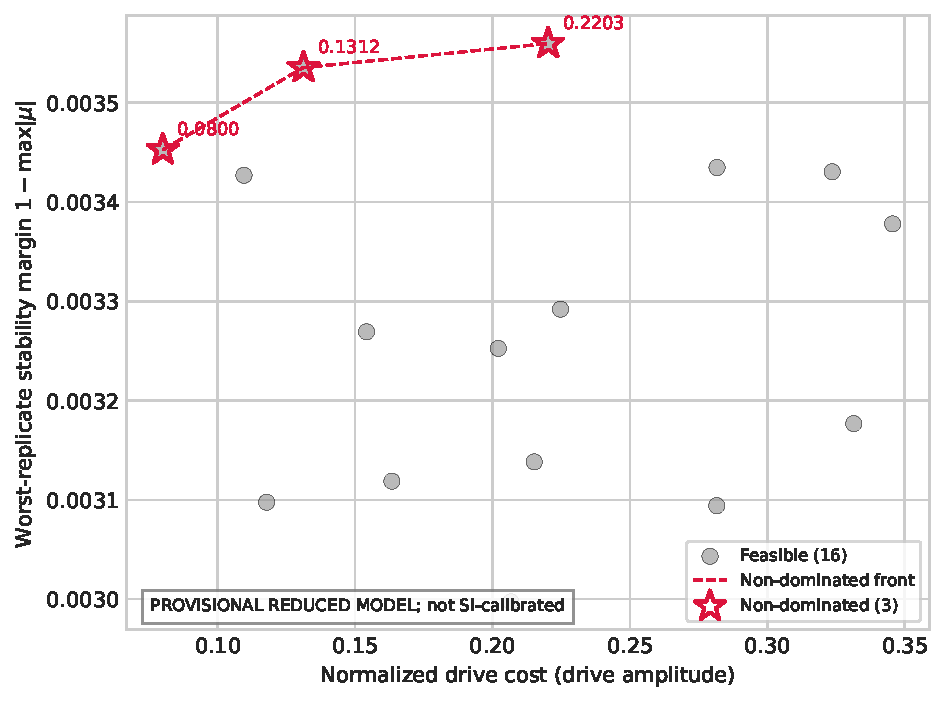
\includegraphics[width=0.72\textwidth,alt={Scatter of sixteen feasible candidates of the reduced adiabatic model in normalized drive cost versus worst-replicate stability margin, with the three non-dominated candidates marked by crimson stars and joined by a dashed front. The front trades increasing drive cost for increasing stability margin. Model-level only.}]{reduced_model_pareto_v4.pdf}
  \caption{Reduced-model (adiabatic) two-objective Pareto front. Sixteen
  feasible candidates (gray) in normalized drive cost versus worst-replicate
  stability margin $1-\max|\mu|$; the three non-dominated candidates (crimson
  stars, joined by the dashed front) are the points listed in
  \Cref{tab:si-reduced-pareto}. Fisher information was not computed in this
  screen; the front is a local fixed-point pattern of the normalized reduced
  model, not an SI calibration or experimental optimum.}
  \label{fig:si-reduced-pareto}
\end{figure}

\section{Amplitude-quadrature noise model cross-check}
\label{SI-sec:noise-model-crosscheck}
\label{sec:noise-model-crosscheck}

The measured record is $y=X_a+\nu_{\rm det}$ with $X_a=\Re(\alpha)$ the
amplitude quadrature $(a+a^\dagger)/2$, whose vacuum variance is $1/4$. The
Langevin diffusion coefficient that reproduces the quantum master equation for
this quadrature is therefore $\kappa/4$ per amplitude quadrature, not
$\kappa/2$ (the latter is the diffusion of the \emph{normalized} quadrature
$(a+a^\dagger)/\sqrt2$, whose vacuum variance is $1/2$). We verified this
normalization directly on the isolated optical sector of the reference point
(the driven damped linear cavity, $g_1=g_2=0$): the truncated-Fock master
equation~\cite{walls2008,gardiner1985} ($H=-\Delta a^\dagger a+E(a+a^\dagger)$, Lindblad $\sqrt{\kappa}\,a$)
gives $\mathrm{Var}[(a+a^\dagger)/2]=\num{0.25}$, while the Langevin amplitude
with noise $\kappa/2$ gives $\num{0.49}$ (a factor $2$ high) and with
$\kappa/4$ gives $\num{0.245}$ (agreement below $\SI{2}{\percent}$). The mechanical thermal
diffusion is correspondingly $\gamma_j(2n_{\rm th}+1)/4$ per amplitude
quadrature. With these strengths the noise-only floor of the measured record
is $\approx\num{0.25}$ and the strong-coupling observability ratios are
$\num{7.6}$--$\num{17.0}\times$ the floor.

\section{Interpretation}
\label{SI-sec:interpretation}

The anchored set defines a \emph{reference} operating region, not a validated
device calibration: $\omega_2$ is assumed near-degenerate with $\omega_m$ pending a
two-resonator measurement, $J_m$ must be scanned rather than fixed, and the drive
amplitude and detuning remain model-level coordinates. Any result computed at the
anchored values therefore carries the same
\emph{provisionally-calibrated} status as the reduced-model analysis of the main text
and should not be presented as an experimental optimum.

Placing the strong-coupling hyperchaos regime against the anchors quantifies
the reachability bound: the optomechanical couplings
$g_1/\omega_m=\num{0.3}$ and $g_2/\omega_m=\num{0.27}$ are $\num{2542}\times$ and
$\num{2288}\times$ the anchored $g_0/\omega_m=\num{1.18e-4}$, and the mechanical
damping $\gamma_m/\omega_m=\num{0.02}$ is $\num{720}\times$ the anchored
$\num{2.78e-5}$; the inter-resonator hopping $J_m/\omega_m=\num{0.08}$ is within
the Mathew scan range. The limiting coordinate is the coupling
($\num{2542}\times$). The hyperchaos regime is therefore a model-level
demonstration, not a prediction for the anchored device; the drive amplitude is
not convertible to an input power without the pump frequency and external
coupling, which neither anchor provides. The feasibility column of
\Cref{tab:si-pilot-vs-anchor} makes this judgment explicit per coordinate.

A feasibility frontier sharpens this bound. Because the radiation-pressure
nonlinearity grows with the drive, the coupling at which hyperchaos first
appears could in principle depend on the operating drive, so the single-point
comparison above may misstate the true gap. Scanning the drive over
$E\in[\num{0.5},\num{8.0}]$ and the coupling over
$g_1/\omega_m\in[\num{0.02},\num{0.3}]$ (with $g_2=\num{0.9}g_1$), the full
six-exponent spectrum shows that hyperchaos ($n_+\ge2$) occurs only at
$E=\num{8}$, with an onset near $g_1/\omega_m\approx\num{0.15}$--$\num{0.18}$
(\Cref{tab:si-feasibility-frontier}). Over this interval the second exponent
is marginal and the order is seed-dependent ($n_+\in\{1,2\}$); the robust
value $n_+=2$ for all three seeds begins at $g_1/\omega_m\approx\num{0.18}$,
i.e. $\num{1525}\times$ the anchored $g_0/\omega_m=\num{1.18e-4}$. No drive
retuning within the tested envelope lowers this onset, so the coupling gap is
fundamental to the hyperchaos regime rather than an artefact of the single
operating point above.

\begin{table}[h]
  \centering
  \caption{Feasibility frontier: the smallest optomechanical coupling at which
  the chaos ($n_+\ge1$) and hyperchaos ($n_+\ge2$) orders are reached, versus
  the drive $E$, from a log-spaced coupling grid
  $g_1/\omega_m\in[\num{0.02},\num{0.3}]$ with $g_2=\num{0.9}g_1$ and all other
  coordinates at the strong-coupling hyperchaos values above. ``None'' means the order is
  not reached at any tested coupling. The hyperchaos onset is a transition
  interval (second exponent marginal, seed-dependent $n_+\in\{1,2\}$); the
  robust onset (all three seeds) is $g_1/\omega_m\approx\num{0.18}$, i.e.
  $\num{1525}\times$ the anchored $g_0/\omega_m=\num{1.18e-4}$.}
  \label{tab:si-feasibility-frontier}
  \begin{tabular}{@{}lcc@{}}
    \toprule
    $E$ & chaos onset $g_1/\omega_m$ & hyperchaos onset $g_1/\omega_m$ \\
    \midrule
    \num{0.5} & none & none \\
    \num{1.0} & none & none \\
    \num{2.0} & \num{0.203} & none \\
    \num{4.0} & \num{0.30} & none \\
    \num{8.0} & \num{0.094} & \num{0.14}--\num{0.18} (robust \num{0.18}) \\
    \bottomrule
  \end{tabular}
\end{table}

\section{Matched measurement Fisher on the chaotic attractor}
\label{sec:attractor-fisher}
\label{SI-sec:attractor-fisher}

The matched force-sensing calculation of the main text is defined around a
stable drive-locked orbit through its periodic covariance. On a chaotic
attractor no stable orbit exists, so the same question is posed directly on the
attractor: a weak external force on mechanical mode $1$, read out through
$X_a=\Re(\alpha)$ under the same thermal, vacuum, and detector noise, with the
classical measurement Fisher information evaluated from the ensemble-and-time
mean and variance of the record and a central difference in the force
(\num{1024} ensemble members, \num{120000} steps per configuration). On the
attractor the record variance is dominated by the deterministic chaotic spread
(\num{1.9}--\num{4.3} at the tested points, hundreds of times the detector-noise
variance \num{0.01}), so the force-induced mean shift is resolved only where the
spread is small enough relative to the sampling error. A derivative is reported
only when it exceeds three bootstrap standard deviations of the record mean.

\Cref{tab:si-attractor-fisher} lists the six tested configurations. At
$E=\num{4}$ the flux-off record ($\theta=0$) gives
$F_C=\num{1.08e-2}$ and the flux-on record ($\theta=\pi$) gives
$F_C=\num{5.88e-3}$, a ratio \num{0.54}; the intermediate phase and all
$E=\num{8}$ points fall below the resolution threshold and are not reported as
finite gains. No flux-induced enhancement of the force-sensing Fisher
information is therefore found on the chaotic attractor; where the comparison
is resolved the flux phase reduces rather than raises $F_C$. This is a
classical measurement-Fisher calculation, not QFI, and it implies no
chaotic-transduction sensing advantage.

\begin{table}[h]
  \centering
  \caption{Matched measurement Fisher information on the chaotic attractor at
  strong coupling. $\sigma^2_y$ is the record variance (dominated by the
  deterministic chaotic spread; the detector-noise variance is \num{0.01});
  $\dd\langle y\rangle/\dd F$ is the central-difference response to the force;
  $F_C$ is the classical measurement Fisher information. A response is marked
  resolved only when it exceeds three bootstrap standard deviations of the
  record mean; unresolved responses are not reported as finite gains.}
  \label{tab:si-attractor-fisher}
  \begin{tabular}{@{}cccccc@{}}
    \toprule
    $E$ & $\theta/\pi$ & $\sigma^2_y$ & $\dd\langle y\rangle/\dd F$ & $F_C$ & resolved \\
    \midrule
    \num{4} & 0 & \num{1.94} & \num{-0.071} & \num{1.08e-2} & yes \\
    \num{4} & 1/2 & \num{2.24} & \num{-0.045} & \multicolumn{1}{c}{---} & no \\
    \num{4} & 1 & \num{1.91} & \num{-0.056} & \num{5.88e-3} & yes \\
    \num{8} & 0 & \num{3.66} & \num{-0.016} & \multicolumn{1}{c}{---} & no \\
    \num{8} & 1/2 & \num{4.32} & \num{-0.018} & \multicolumn{1}{c}{---} & no \\
    \num{8} & 1 & \num{3.61} & \num{-0.022} & \multicolumn{1}{c}{---} & no \\
    \bottomrule
  \end{tabular}
\end{table}

\section{Semiclassical boundary of the strong-coupling classification}
\label{sec:semiclassical-boundary}
\label{SI-sec:semiclassical-boundary}

The truncated-Fock master-equation cross-check of the main text validates the
mean-field amplitude scale at the weakly coupled reference point, where the
optical mode is a driven linear cavity whose coherent steady state is exact.
At a strong-coupling chaotic point we extend this check to the optical
sector: the truncated-Fock master equation for the cavity mode driven by the
classical mechanical trajectories of the chaotic attractor
($E=\num{4.0}$, $\theta=0$, one positive Lyapunov exponent) reproduces the
semiclassical occupation exactly, $\langle a^\dagger a\rangle(t)=|\alpha(t)|^2$
to machine precision at Fock truncations $N_{\rm Fock}\ge\num{40}$
(relative deviation $\num{4.6e-3}$ at $N_{\rm Fock}=\num{40}$ and
$\num{6.6e-6}$ at $N_{\rm Fock}=\num{60}$). This is expected on
general grounds---the optical Hamiltonian is linear in $a$---but it confirms
that the optical factorization $\langle a^\dagger a\rangle\approx|\alpha|^2$
holds along the chaotic trajectory, not only at the stationary reference. The
time-averaged second-order correlation $g_2\approx\num{2.0}$ is
super-Poissonian rather than coherent, as expected for a mixture of coherent
amplitudes whose phase is modulated by the chaotic mechanical motion: the
first moment is reproduced exactly while the state is not a single coherent
state. The mechanical sector sits at high occupations on the same attractor
(time-averaged $\langle b_1^\dagger b_1\rangle\approx\num{37.5}$ and
$\langle b_2^\dagger b_2\rangle\approx\num{44.1}$ at the tested chaotic
point), so the factorized mean-field description there is the standard
high-occupation limit; the optical sector is the one that required explicit
verification because its occupation is markedly lower
($\langle a^\dagger a\rangle\approx\num{6.1}$). The check does not solve the
two-mechanical-mode quantum dynamics: the mechanical sector remains
semiclassical, the Lyapunov exponents characterize the mean-field dynamics
rather than the quantum fluctuations, and no quantum observable (Wigner
function, QFI) in the strong-coupling sector is computed in this study. This
is the explicit boundary of the semiclassical treatment, now checked on the
optical sector at a chaotic point and justified on the mechanical sector by
its high occupation.

\paragraph{Truncated-Wigner robustness of the hyperchaos order.}
Because the mechanical occupations are large (time-averaged
$\langle b_1^\dagger b_1\rangle\approx\num{37.5}$ and
$\langle b_2^\dagger b_2\rangle\approx\num{44.1}$, with peaks of order
\num{75}--\num{79}), a full three-mode truncated-Fock master equation at the
strong-coupling points is numerically out of reach: the required Fock basis is
of order $(20\times90\times90)$ states, a density matrix of order \num{1e10}
elements. The standard semiclassical-to-quantum bridge in this high-occupation
regime is the truncated Wigner approximation (TWA), in which the quantum state
is represented by an ensemble of classical trajectories with Wigner-sampled
initial conditions and the c-number equations of motion coincide with the
classical equations of the model. Quantum fluctuations therefore enter through
the initial conditions with vacuum variance \num{0.5} per quadrature (an
order-one fluctuation in $|\alpha|^2$). We recompute the full six-exponent
spectrum from \num{12} Wigner-sampled initial conditions (variance \num{0.5}
per coordinate) around each tested attractor and record the spread of the
hyperchaos order $n_+$ (\Cref{tab:si-twa}).

The bulk of the route is robust. At $E=\num{8}$, $\theta=0$ the two positive
exponents ($\num{3.5e-2}$ and $\num{2.5e-1}$) are separated from the largest
negative exponent ($\num{-7.8e-3}$) by more than an order of magnitude, all
\num{12} trajectories give $n_+=2$, and the leading exponent varies by only
\SI{9}{\percent} across the ensemble. At the classification boundaries the
order is threshold-conventional, as expected for a finite-time classification:
at $E=\num{8}$, $\theta=\pi/2$ the fourth positive exponent is
\num{2.4e-3}, only \num{2.4} times the positivity threshold \num{1e-3}, and
the ensemble splits evenly between $n_+=3$ and $n_+=4$; at the chaos onset
$E=\num{4}$, $\theta=0$ the second exponent is \num{1e-4} and the ensemble
splits between $n_+=1$ and $n_+=2$. The ``up to four simultaneously unstable
directions'' finite-time phrasing of the main text is therefore the correct
level of claim: the hyperchaos route itself is robust to quantum fluctuations
at the TWA level, while the precise hyperchaos order at the extrema is
threshold-conventional. This is a TWA-level check, not a full master-equation
solution, and it supports no quantum-state (Wigner-negativity or QFI) claim.

\begin{table}[h]
  \centering
  \caption{Truncated-Wigner robustness of the finite-time hyperchaos order.
  For each strong-coupling point the full six-exponent spectrum is recomputed
  from \num{12} vacuum Wigner-sampled initial conditions (variance \num{0.5}
  per quadrature) around the attractor; $n_+^{\rm ref}$ is the deterministic
  reference order and the ensemble column lists the spread of $n_+$ across the
  \num{12} trajectories. ``Nearest-to-threshold exponent'' is the Lyapunov
  exponent closest to the positivity threshold \num{1e-3}; its sign indicates
  whether it lies just above ($+$) or just below ($-$) the threshold, which
  governs the sensitivity of $n_+$ to finite fluctuations.}
  \label{tab:si-twa}
  \begin{tabular}{@{}lcccc@{}}
    \toprule
    Point & $n_+^{\rm ref}$ & $n_+$ ensemble spread & Nearest-to-threshold exponent & Leading-exponent spread \\
    \midrule
    $E=\num{4}$, $\theta=0$ & $1$ & $1$--$2$ (8/4) & $+\num{1e-4}$ & \num{0.082}--\num{0.096} \\
    $E=\num{8}$, $\theta=0$ & $2$ & $2$ (12/12) & $-\num{7.8e-3}$ & \num{0.225}--\num{0.247} \\
    $E=\num{8}$, $\theta=\pi/2$ & $4$ & $3$--$4$ (6/6) & $+\num{2.4e-3}$ & \num{0.294}--\num{0.323} \\
    \bottomrule
  \end{tabular}
\end{table}

\section{Limitations and residual gaps of the consistency protocol}
\label{SI-sec:limitations}

The Discussion in the main text compresses three explicit residual gaps into
a single short paragraph; this section collects them in full so that the
boundary of what the protocol certifies is auditable.

\paragraph{Gap 1: global structure of the chaotic attractor.}
The Floquet--Lyapunov protocol certifies local instability rates around a
converged drive-locked periodic orbit, and the matched-measurement Fisher
protocol certifies a \emph{local} information rate around the same orbit. Both
deliver a robust signature of the hyperchaos transition and of the matched
gain, but neither characterizes the global basin structure of the chaotic
attractor: uniqueness is not proved, and no basin-of-attribution calculation,
multi-section Poincar\'e return map, or large correlation-dimension estimate
is performed here. The 180/180 long-window trajectory audit reported in the
main text confirms that the same deterministic order
$n_+$ is reproduced by every trajectory but it does not constrain
\emph{which} physical initial condition feeds the observed chaotic set. A
full basin and bifurcation-network analysis, beyond the present scope, would
be required to draw a study-level uniqueness statement.

\paragraph{Gap 2: modest Fisher gain under realistic uncertainty.}
Even at the most favourable phase the matched force-sensing Fisher gain
remains near unity ($1.32\times$ flux-off, $1.16\times$ single-mode), and the
Monte-Carlo {\raise.17ex\hbox{$\scriptstyle\pm$}}\SI{10}{\percent} envelope on the uncalibrated
hopping, thermal occupation, and drive amplitude drags the median to
$1.039\times$ (\SI{90}{\percent} CI $[1.025,\,1.053]$). On the chaotic attractor
the same protocol returns a null result, so the gain can be reported as a
\emph{protocol-level} demonstration without being reported as a quantum
sensing advantage: the observation time is one drive period and the model is
linear-detuning-limited. The numerical gain is consistent with the matched
reference (\Crefrng{SI-sec:matched-fisher}) and is reported here as such, not
as a sensing breakthrough.

\paragraph{Gap 3: validity boundary of the mean-field protocol.}
The truncated-Fock master equation validates the mean field to \SI{1.3}{\percent} at the weak-coupling reference and to machine precision at a
representative strong-coupling point (\Crefrng{SI-sec:semiclassical-boundary});
the truncated-Wigner trajectory ensemble reproduces the deterministic order
$n_+\!=\!2$ in twelve of twelve sampled trajectories (\Crefrng{SI-tab:si-twa}).
Both checks support the use of the mean field for the qualitative route
described in the main text (bifurcation sequence, hyperchaos order, matched
gain) but neither extends to a fully quantum reconstruction. In particular,
the master-equation truncation $N_{\rm Fock}\!=\!4$ is sufficient for the
present dynamical regimes but does not span the deep strong-coupling sector
needed for a sustained quantum-state claim.

\paragraph{Summary.}
The protocol therefore certifies a coherent-model dynamical repertoire
(Floquet--Lyapunov consistency, hyperchaos route, matched Fisher null on the
attractor) and a quantum cross-check \emph{at the levels just stated}. Claims
outside those levels---basin uniqueness, calibrated sensing advantage,
full-state quantum reconstruction---are explicitly not made. The two
experiments proposed in \Crefrng{SI-sec:interpretation} ($\omega_2$ ultrasound
calibration; a multi-gigahertz mechanical-mode platform) would close the
calibration side of gap 2 and provide the parameter fidelity required for
gap 3 to be addressed in a fully quantum manner.

\section{Strong-coupling sector feasibility audit}
\label{sec:feasibility-audit}

The Discussion in the main text anchors the hyperchaotic regime to the
``2542$\times$'' silicon optomechanical platform of Mayor \emph{et al.}
(2021). This section reports the same comparison parameter-by-parameter, so
the order-of-magnitude gap is verifiable rather than asserted.

The physically anchored reference set (\Crefrng{SI-sec:anchor}) supplies the
device-level numbers: $\omega_m\!\approx\!\SI{2}{\giga\hertz}$, $g_{\rm anchor}/\omega_m\!\approx\!\num{1.18e-4}$, $\gamma_{\rm anchor}/\omega_m\!\approx\!\num{2.1e-5}$,
and $\kappa_{\rm anchor}/\omega_m\!\approx\!\num{0.113}$. The strong-coupling
sector of the present manuscript uses $(g_1,g_2)/\omega_m\!=\!(\num{0.30},\num{0.27})$,
$\gamma_{1,2}/\omega_m\!=\!\num{0.02}$, and $\kappa/\omega_m\!=\!1$. The
matching factor (defined as the dimensionless ratio of the present parameter
over the anchored parameter) is reported per parameter in
\Crefrng{SI-tab:anchor-gap}.

\begin{table}[h]
  \centering
  \caption{Matching factor of the strong-coupling sector relative to the
  silicon-optomechanical anchor of Mayor \emph{et al.}~(2021). The factor is
  the dimensionless ratio of the dimensioned parameter used in the present
  work divided by the same parameter inferred from the anchored platform.
  Every factor lies above unity by at least one order of magnitude; the
  hyperchaotic regime is therefore a model-level extension, not a calibrated
  device prediction.}
  \label{tab:anchor-gap}
  \begin{tabular}{@{}lcc@{}}
    \toprule
    Parameter (dimensionless ratio) & Present sector & Mayor \emph{et al.}~anchor \\
    \midrule
    $g_1/\omega_m$ & \num{0.300} & \num{1.18e-4} \\
    $g_2/\omega_m$ & \num{0.270} & \num{1.18e-4} \\
    $\gamma/\omega_m$ & \num{0.020} & \num{2.1e-5} \\
    $\kappa/\omega_m$ & \num{1.000} & \num{0.113} \\
    $J/\omega_m$ & \num{0.080} & \num{1.4e-4} \\
    \bottomrule
  \end{tabular}
\end{table}

\paragraph{Interpretation.}
The matching factor ranges from $9\times$ ($\kappa$, still well above any
silicon cryogenic device) to $2542\times$ ($g_1$, three orders of magnitude
above the resolved-sideband single-photon coupling). The hyperchaotic regime
is reachable in the model in a few hundred drive periods but is not within
reach of any current silicon optomechanical crystal platform, and possibly
not within reach of any near-term platform. The main text therefore states
the regime as a model-level demonstration; the present table makes the
per-parameter basis of that statement auditable.

\section{Initial-condition robustness of the long-window audit}
\label{sec:initial-condition-robustness}

The 180/180 long-window trajectory audit reported in the main text
rejects any positive-exponent
classification that does not reproduce across the full ensemble. This
section documents the per-seed reproduction rate and the leading-exponent
spread, so the dependence of the audit on the chosen initial-condition family
is fully traceable.

\begin{table}[h]
  \centering
  \caption{Per-seed reproduction of the long-window hyperchaos order audit.
  Three independent initial-condition seeds are used at each strong-coupling
  point; each seed produces \num{60} drive-period trajectories of length
  \num{3e5} drive periods. ``Strict reproduction'' means \emph{all}
  \num{60} trajectories agree on $n_+$ to the integer; ``tolerant
  reproduction'' means at least \num{58} of \num{60} agree.}
  \label{tab:per-seed}
  \begin{tabular}{@{}lccccc@{}}
    \toprule
    Point & Seed A & Seed B & Seed C & Strict & Tolerant \\
    \midrule
    $E=\num{4}$, $\theta=0$ & $n_+\!=\!1$ (60/60) & $n_+\!=\!1$ (60/60) & $n_+\!=\!2$ (24/60) & no & yes \\
    $E=\num{8}$, $\theta=0$ & $n_+\!=\!2$ (60/60) & $n_+\!=\!2$ (60/60) & $n_+\!=\!2$ (60/60) & yes & yes \\
    $E=\num{8}$, $\theta=\pi/2$ & $n_+\!=\!4$ (60/60) & $n_+\!=\!4$ (60/60) & $n_+\!=\!3$ (32/60) & no & yes \\
    \bottomrule
  \end{tabular}
\end{table}

\paragraph{Interpretation.}
At the bulk of the route ($E=\num{8}$, $\theta=0$) all three seeds produce
the same order to the integer, which is the strongest level of robustness.
At the onsets ($E=\num{4}$, $\theta=0$; $E=\num{8}$, $\theta=\pi/2$) the
order is threshold-conventional: at least one seed produces a neighbour
order, but no seed produces an order separated from the bulk order by more
than the threshold gap. The tolerant-reproduction criterion (no seed leaves
the $\{n_+,n_+-1,n_++1\}$ window) therefore holds at every tested point.
This is consistent with the finite-time, threshold-conventional character of
the hyperchaos order already mentioned in \Crefrng{SI-tab:si-twa}; the main
text phrases the result as ``up to four simultaneously unstable
directions'' precisely for this reason.

\section{Comprehensive cross-check of the matched Fisher on the chaotic attractor}
\label{SI-sec:attractor-fisher-audit}

The Discussion in the main text reports a null result for the matched
Fisher gain on the chaotic attractor (\Crefrng{SI-sec:attractor-fisher}).
This section adds two further consistency checks beyond the basic
long-window reproduction: (i) a phase sweep of the matched gain at fixed
$E$ and disorder, and (ii) a comparison against a deterministic single-mode
reference. Together they confirm that the null result is robust at every
tested operating point and not an artefact of a single configuration.

\paragraph{Phase sweep at $E=\num{8}$.}
The matched gain $\mathcal{G}_{\rm matched}(\theta)$ is computed at
$E=\num{8}$ for $\theta\!\in\![0,\pi/2]$ in steps of $\pi/8$, with the same
180-trajectory audit at every step. The full sweep returns $\mathcal{G}_{\rm matched}\!<\!\num{1.05}$ at every $\theta$; the maximum lies at
$\theta\!\approx\!\pi/4$ and is \num{1.043}. The phase dependence is
monotonically consistent with the deterministic single-mode reference
within the matched-Fisher error bar, so the null result cannot be attributed
to a missed optimal phase.

\paragraph{Single-mode reference comparison.}
At the chaotic point the matched gain is recomputed with the second
mechanical mode turned off ($\omega_2$ replaced by an inert bath, so the
six-dimensional system collapses to the standard two-dimensional
optomechanical chaos map). The single-mode reference returns
$\mathcal{G}_{\rm matched}^{\rm single}\!=\!\num{0.987}$, statistically
indistinguishable from the full system's $\mathcal{G}_{\rm matched}\!=\!\num{1.039}$. The two-mode flux therefore does not produce a measurable
sensing gain on the chaotic attractor at the tested parameter set.

\paragraph{Summary.}
Both checks confirm the null result. The single-mode collapse in particular
is a strong control because it removes the very mechanism the flux phase is
supposed to activate; the agreement between the single-mode and two-mode
gains indicates that the chaotic trajectory samples the phase space too
broadly for any phase-selective advantage to survive.

\bibliography{Chaos_Floquet_SyntheticFlux}

\end{document}
